\chapter{Background}
\label{Background}

This chapter gives an outline of the concepts and a detailed explanation of the various technologies that will be used later in this thesis.

	\section{Containers}
	\label{Background:Containers}
	The concept of container technology uses the same model as shipping containers in transportation. The idea is that before the invention of shipping containers, manufacturers had to ship goods in a variety of fashions which included ships, trains, airplanes, or trucks, all with different sized containers and packaging.
	With the standardization of shipping containers, products could be transported seamlessly without further preparation using different shipping methods. Before the arrival of this standard, shipping anything in volume was a complex, laborious process. The motivation behind software containers is the same. \cite[P.~1]{Kinnary2018}\\

	Instead of shipping a complete operating system (OS) and the software (with necessary dependencies), we pack our code and dependencies into an image that can run anywhere. Furthermore,  it enables the packaging of clusters of containers onto a single computer. In other words, a container consists of an entire runtime environment: an application, plus all the dependencies, libraries, and other binaries, and configuration files needed to run it, bundled into one package.
	The ability to have software code packaged in pre-built software containers means that code can be pushed to run on servers running different Linux kernels or be connected to run a distributed app in the cloud. This approach also has the advantage of speeding up the testing process and creating large, scalable cloud applications. This approach has been in software development communities for several years. It has recently gained in popularity with the growth of Linux and cloud computing. \cite[P.~2]{Kinnary2018}\\
	
	% \newpage
	\subsection{Containerization vs Virtualization}
	Linux containers and virtual machines (VMs) are both package-based computing environments that combine several IT system components and keep them isolated from the rest of the system. Their main distinguishing features are scalability and portability. Containers are usually measured in megabytes, whereas VMs in gigabytes.
	\cite{containersRedHat}
	\begin{figure}[H]
		\centering
		% \input{"Bilder/tikz/Grundlagen/docker-types-of-mounts.tex"}
		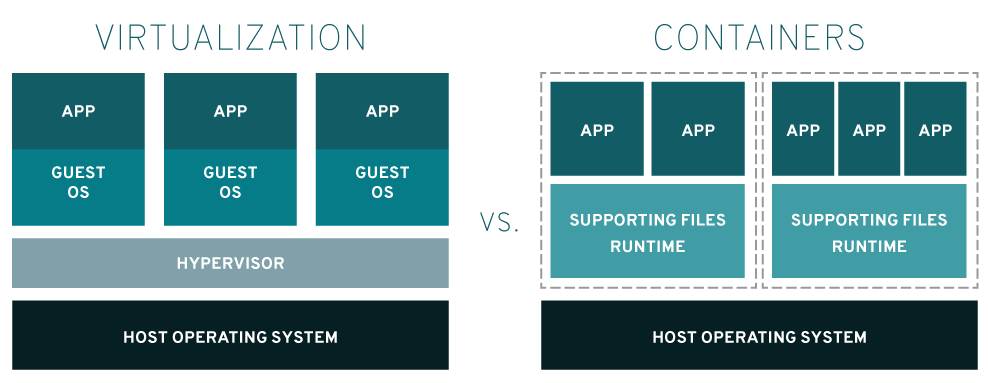
\includegraphics[width=0.9\textwidth]{"Bilder/virtualization-vs-containers_transparent.png"}
		\caption{Differences between Virtualization and Containerization \cite{containersRedHat}}
		\label{fig:Background:Containers:Containers vs VMs}					
	\end{figure}

	\paragraph*{Containerization} is an alternative to standard virtualization that encapsulates an application in a container with its executing environment.
	Containers hold an application and everything it needs to run. Everything within a container is maintained on an image—a code-based file that includes all libraries and dependencies. These files are similar to a Linux distribution installation. An image comes with RPM packages and configuration files. Containers are so small compared to VMs, there are usually hundreds of them loosely coupled together.\cite{containersRedHat}
	
	\paragraph*{Virtualization} is a way of sharing a single physical instance of a resource or an application to multiple organizations and clients. It utilizes software called a hypervisor that separates resources from their physical devices. It enables the partitioning of the resources and assigned to individual VMs. When a user issues a VM instruction that requires additional resources from the physical environment, the hypervisor sends the request to the physical system and saves the changes. VMs look and act like physical servers, which can multiply the drawbacks of application dependencies and large OS footprints—a footprint that's often not required to run a single app or microservice.\cite{containersRedHat} \\

	Table \ref{tab:container_vs_vms} illustrates the key differences between the above two approaches concerning package-based computing environments.
	\begin{table}[H]
        \centering
		\rowcolors{1}{}{gray!25}
        \begin{tabular}{{p{3cm}|p{5cm}|p{6cm}}}
            \toprule
            Parameters & Virtualization & Containerization\\
            \midrule
            Isolation & Provides complete isolation from the host operating system and the other VMs & Provides lightweight isolation from the host and other containers, but doesn’t provide a strict security boundary as a VM \\
            Operating System & Runs a complete operating system including the kernel, thus requiring more system resources such as CPU, memory, and storage & Runs the user-mode portion of an operating system, and can be customized to include just the required services for your app utilizing fewer system resources \\
            Compatibility & Runs just about any operating system inside the virtual machine & Runs on the same operating system version as the host\\
            Deployment  & Deploys individual VMs by using Hypervisor & Deploys single container by using Docker or deploy multiple containers by using an orchestrator such as Kubernetes\\
            Persistent storage  & Uses a Virtual Hard Disk (VHD) for local storage for a single VM or a Server Message Block (SMB) file share for storage shared by multiple servers & Uses local disks for local storage for a single node or SMB for storage shared by multiple nodes or servers\\
            Networking  & Uses virtual network adapters & Uses an isolated view of a virtual network adapter. Thus, providing a little less virtualization\\
            Startup time & They take few minutes to boot up & They can boot up in few seconds \\
            \bottomrule
        \end{tabular}
		\caption{Differences between Virtualization and Containerization \cite{containers-vs-vms-Baeldung}}
		\label{tab:container_vs_vms}
    \end{table}

	The use of containers can decrease the required time for developing, testing, and deploying applications. It makes testing and fault detection less complex as there is no difference between running your application on a test environment and in production. It provides a cost-effective solution and can help reduce operational and development expenses. In most use-cases, container-based virtualization offers several advantages over traditional Virtual Machine based virtualization.

	\section{Docker}
	\label{Grundlagen:Docker}
	\textit{Docker is a person who works at a port whose job is to load goods onto and off container ships.} \cite{docker-definition-english}

	Software Docker essentially does the same in the software context. Docker is a collection of open-source tools that quickly wraps up any application and all its unique dependencies in a lightweight, portable, self-sufficient container that can run virtually anywhere on any infrastructure.\cite{docker-definition}
	Docker was launched as an open-source project by dotCloud, Inc. in
	2013. it relies heavily on namespaces and cgroups to provide resource isolation and to package an application along with its dependencies. This bundling of dependencies into one package allows an application to run across different platforms and still support a level of portability. This provides flexibility to developers to develop in the desired language and platform. It has drawn a lot of interest in recent years.\cite[P.~10]{Kinnary2018}

	Docker consists of several parts. The following section gives an overview of the main components of Docker.


		\subsection{The Docker Runtime and Orchestration Engine (Docker Engine)} 
		\label{Grundlagen:Docker:Docker Engine}
		The Docker engine is the software for the infrastructure that runs and orchestrates containers. All other Docker, Inc. and third-party products connect to and develop around the Docker Engine. It provides a workflow for building and managing the application stack. It builds and runs containers using other Docker components and services. It consists of the Docker daemon; a REST API that specifies the interfaces that programs can use to communicate with the daemon; and the CLI, the command-line interface that communicates with the Docker daemon via the API. Docker Engine creates and runs the Docker container from the Docker image file.\\
		\\
		Following Diagramm illustrates the Docker System Architecture.
		\begin{figure}[H]
			\centering
			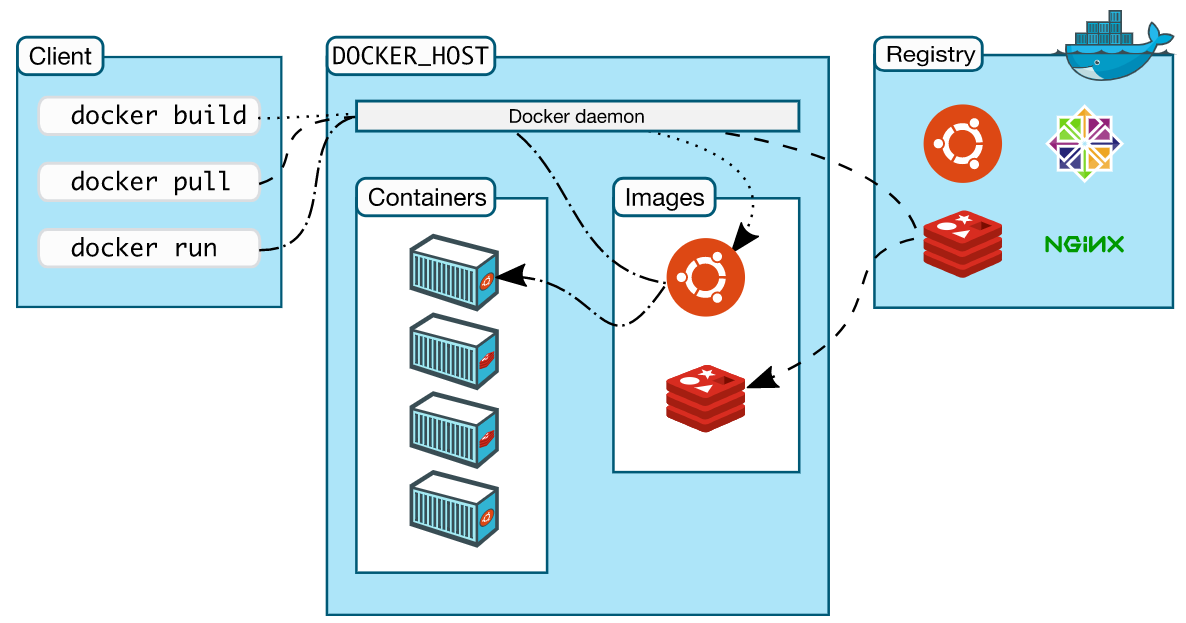
\includegraphics[width=0.9\textwidth]{"Bilder/DockerArchitecture.png"}
			\caption{Docker System Architecture \cite{dockerOverwiew}}
			\label{fig:Background:DockerEngine:Architecture}					
		\end{figure}

		\paragraph{Docker daemon (dockerd)}  is a server process that runs
		in the background. It continuously listens to the REST API interface
		and listens for incoming requests and manages Docker objects (images, containers, networks, and volumes).  A daemon also has the ability to communicate with other daemons to manage Docker services.\cite{dockerOverwiew}

		\paragraph{Docker client} represents the primary means for most users to interface with Docker. The commands run through the command-line interface are sent to the Docker daemon through the Docker API interface. The Docker daemon(dockerd) then executes these commands. The Docker client has the ability to connect with multiple Docker daemons.\cite[P.~32]{Kinnary2018}
		
		\paragraph{Docker registry} The images created by the Docker daemon are stored in the Docker registry. Docker looks for images in the Docker Hub by default, but it is possible to have a self hosted private registry. Docker Hub is a public registry and is freely accessible.\cite[P.~33]{Kinnary2018}
			
		\subsection{Docker Objects}
		\label{Grundlagen:Docker:Docker Objects}
		\paragraph{Images}
		A Docker image is a read-only file system that contains instructions to create a container in which an application can run. In most cases, a Docker Image is based on another image and is customized. You can either use existing images published in public repositories such as Docker Hub or Create your image.
		A Dockerfile is used to create a Docker image. A Dockerfile contains simple instructions that can be understood by the Docker daemon to	create the image and run it. Docker images are layers that correspond to each instruction in the Dockerfile. Part of what makes a Docker image super easy is that when you change a part of the Dockerfile, only that layer is changed, and not the entire image.

		\paragraph{Containers}
		A Docker container is an instance of an image. An image runs inside a container. You can manage a container with the stop, start, and delete commands to manage it. Multiple containers can be connected over a network. They can be connected to the memory, and they can also communicate with each other. Containers are much more lightweight than VMs because their startup times are very fast. To create a container, in addition to the container's configuration and settings, you also create an image Configuration and settings an image is created. When a container is deleted everything related to the container is also deleted, including state and memory.

		\paragraph{Services}
		In a distributed application, different functionalities of the app provide different services. For example, if you are building an application that suggestions based on keywords that the user enters, you might want to have A front-end service that takes the word and sends it to the service that will Verifies the legitimacy of the word. This in turn could be sent to another service that runs an algorithm to generate the suggestions, etc., which are then returned to the service. These are all different services on different Docker containers, sitting Sit behind different Docker daemons. These Docker daemons are all connected over the network and interact with each other.
		All these services work together as a swarm, managed by different Managers and workers to manage. Each swarm contains a Docker daemon. These Daemons communicate with each other using the Docker API. A Docker Compose YAML file is used to get all these services running together. together to get them running. 

		\paragraph{Networks}

		\paragraph{Volumes}
			
			
		\paragraph{Dockerfiles}
		Dockerfile is a text document that contains a set of instructions or commands for assembling an image that is understood by the build engine. The Dockerfile defines what goes into the environment inside your container. Accessing resources, mapping volumes, passing arguments, copying files that need to be inside your container are defined in this file. According to Dockerfile created, you need to build it to create the image of the container. Create container image. The image is just a snapshot of all the executed statements in the Dockerfile. Once this application image is created, you can expect that it will run on any machine that uses the same kernel. 
		
		\paragraph{Docker-Compose}
		Docker Compose is the tool for running multi-container Docker applications. It is essentially a YAML file that can be thought of as a Compose of multiple Dockerfile containers, which can be used to put commands into a single file. This Docker Compose YAML file contains configurations of multiple services. Then, with a single command, you can run all services to run in Docker containers at the same time.
		Docker Compose can be used to create a microservices architecture and link the containers together, or it can be used for a single service. In addition, Docker Compose can create images, scale containers, and re-run containers that have been stopped. All of these functions are part of Docker. Docker-compose is just a higher-level abstraction of container execution commands. Everything that a compose file can do, can likewise be performed with simple Docker commands, except that this requires more memory and additional overhead to execute any additional commands, to connect to the network, etc. . Docker-compose helps to simplify this process.
				
	\section{Industrial Edge}
	\label{Grundlagen:IndustrialEdge}
		
	Industrial Edge is a development from Siemens that makes it possible to analyze data generated in various industrial processes on the device itself. It combines local engineering with cloud engineering.\cite{siemensIndustrialEdge}

	This eliminates unnecessary data transport between the end device and the server, only processed data is sent to the server. The processing load is in this way directed from the server towards the end device. Edge applications serve this purpose, they contain a fixed set of functions and can be accessed with the edge infrastructure on the respective end device (edge device). These apps are based on Docker technology and run one or more Docker containers in them. Figure \ref{fig:Grundlagen:IndustrialEdge:Ueberblick} shows a typical infrastructure from the top server to the end devices.

		\begin{figure}[h]
			\centering
			%\input{"Bilder/tikz/Grundlagen/industrial-edge-overwiev.tex"}
			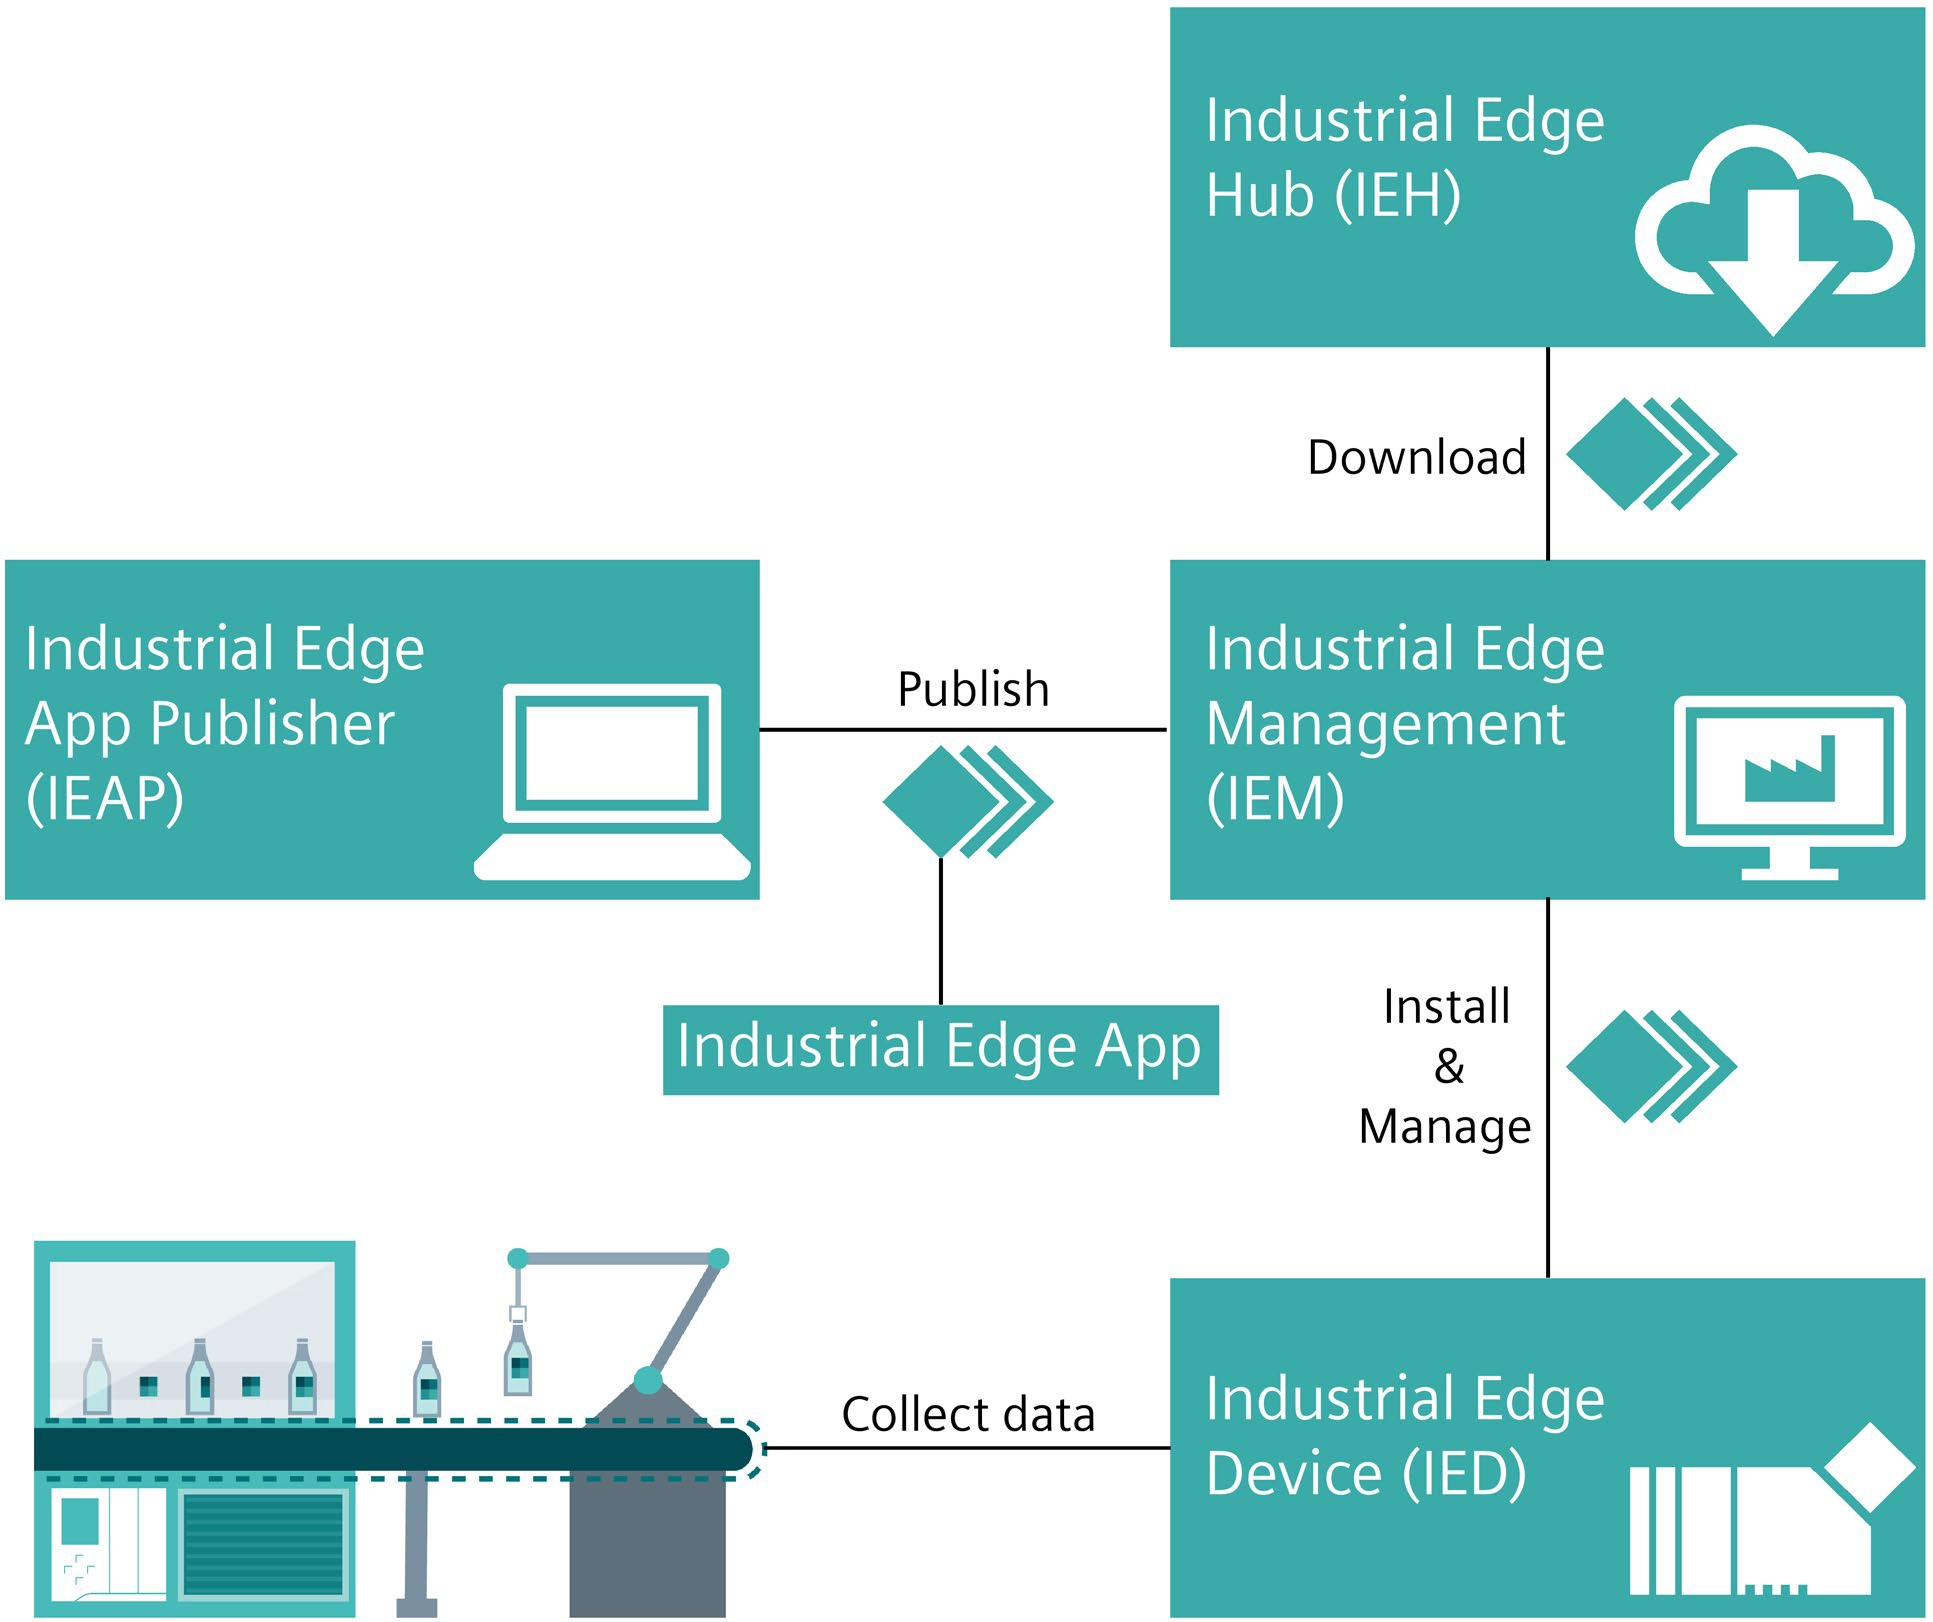
\includegraphics[width=0.70\textwidth]{"Bilder/Edge_uebersicht.jpg"}
			\caption{Industrial Edge overview \cite{siemensIEM_gettingStarted}}
			\label{fig:Grundlagen:IndustrialEdge:Ueberblick}					
		\end{figure}
	
		%- Management tool für Docker Container auf Geräten (Device)\\
		%- Graphen die das IE-Hub, IEM, Docker Device erklärt\\
			
		\paragraph{Industrial Edge Management System}
			The \gls{IEM} is a server, which can be operated independently in a local network. It allows the user to create their own server which avoids the transmission of raw sensitive data exchanged between the edge device and the IEM over the Internet.

			In addition, the end(edge) devices can be managed via this server, which includes the installation of apps and software updates and further analysis of individual apps. A self-developed Application can be uploaded to the IEM, which in turn can distribute it to the edge devices.\cite{siemensIndustrialEdge}

		\paragraph{Industrial Edge Hub}
			The \gls{IEH} 
			is the top server-level Application hub provided by Siemens. On this platform, Siemens offers applications developed in-house. These can be loaded onto the IEM for a license fee. Any required software packages and documentation can be downloaded from here. This streamlines the development process of custom applications including deployment, and operation on desired IEM.\cite{siemensIndustrialEdge}
		\paragraph{Industrial Edge App}
			An \gls{IEA} (edge app) is used for the intelligent processing of industrial automation tasks.\cite{siemensIndustrialEdge} It is a Docker-based image, which is runs on the IED. A docker-compose file acts as the top description level file, it specifies various parameters and the sequence in which the Docker images are started. The parameters include network configuration, data storage, and other application-specific configurations. It supports all Docker-compose version 2.4 settings. Modification of this docker-compose file allows configuring any Edge app, even after it has been already downloaded to an edge device. An Edge App can be downloaded to an edge device through the IEM.
	
		\paragraph{Edge Device}
		Edge devices are required in order to run individual edge apps. The edge device is a custom Linux Machine running the Industrial Edge OS. For test and simulation purposes it can also be run in a Virtual machine(VM). Edge devices can save automation data locally and retrieve it when required. In addition, edge devices can upload this data into the cloud infrastructure and retrieve it at any moment. After proper configuration and connection,  an Edge Device can be activated through IEM using an Edge Device configuration file.
			
		\paragraph{Industrial Edge Publisher}
		The Industrial Edge Publishers is a tool that converts Docker images into Edge Apps and uploads them to the IEM. It can also be used to manage, modify or delete apps that have already been created.\cite{siemensIE_App} A prerequisite for creating an app is a docker-compose file, which contains the startup parameters of a Docker container. These parameters can also be configured through a menu within the Edge Publisher.
			

	
	\section{ROS}
	\label{Grundlagen:ROS2}		
	This chapter covers the basics of the robot operating system (ROS) and all the tools necessary to create, debug, and understand robot applications. This chapter describes some high-level concepts and low-level API commands which enable developers to develop, maintain and support multi-robot applications. \\
	
	The software stack of a typical robot system requires several software tools which include hardware drivers, network modules, communication architecture, and several application-specific algorithms. ROS provides these tools in one package, which saves developers a lot of time and redundant work. ROS includes several sub-packages for robot navigation, vision, control, simulation.\\
	
	The Robot Operating System (ROS) has long been one of the most widely used middleware for robotic. The large open-source robotics community has contributed to a lot of new features since the introduction of ROS 1 in 2007, limitations of ROS1 have led to the development of ROS2.\cite{ros2Basic}\\

	\subsection{ROS2} 
	\label{Grundlagen:ROS:ROs2}
	\gls{ROS2} was launched with an improved architecture and upgraded features. It is new and various organizations and open-source communities are trying to port existing packages to ROS 2.\cite{ros2Basic} \\
	
	Table \ref{tab:ros1_vs_ros2} illustrates the key differences between ROS1 and ROS2
	\begin{table}[H]
        \centering
		\rowcolors{1}{}{gray!25}
        \begin{tabular}{{p{3cm}|p{5cm}|p{6cm}}}
            \toprule
            Parameters & ROS1 & ROS2\\
            \midrule
            Networking & Utilizes the TCPROS communication protocol & Uses DDS (Data Distribution System) for communication.\\
            ROS Master & Uses ROS Master for centralized discovery and registration. The whole communication system fails if the master fails. & Uses the distributed DDS discovery. ROS 2 provides a custom API to get all information about nodes and topics. \\
            Compatibility & ROS runs only in Ubuntu. & ROS 2 is compatible with Ubuntu, Windows 10, and OS X.\\
            Programming language  & Uses C++ 03 and Python2. & Uses C++ 11 and Python3.\\
            Build system  & ROS uses only the CMake build system and has a combined build for multiple packages via a single CMakeLists.txt file & ROS 2 offers options to use other build systems. Supports isolated independent builds for packages to better handle dependencies between packages.\\
            Default values & Data types in message files do not support default values. & Data types in message files support default values.\\
            roslaunch & roslaunch files are written in XML. & roslaunch files are written in Python which makes it more configurable and and supports conditional execution.\\
            Realtime Support & Does not support Real-time behavior. & Supports real-time responses with a suitable RTOS.\\
			\bottomrule
        \end{tabular}
		\caption{Differences between ROS1 and ROS2 \cite{ros1vsros2}}
		\label{tab:ros1_vs_ros2}
    \end{table}

	\subsection{ROS2 Structure}
	\label{Grundlagen:ROS2:ROS2_Structure}
	The key ROS2 feature is that it uses DDS (Data Distribution System) for communication. It eliminates ROS Master and utilizes distributed DDS discovery.	A set of related nodes located on the same computer are called a hub, where one or more hubs can be present on the same computer. ROS hubs are considered to have an accompanying set of bridging nodes that pass messages between ROS and ROS2.\cite*[P.7]{Koubaa2021}
	\begin{figure}[H]
		\centering
		% \input{"Bilder/tikz/Grundlagen/docker-types-of-mounts.tex"}
		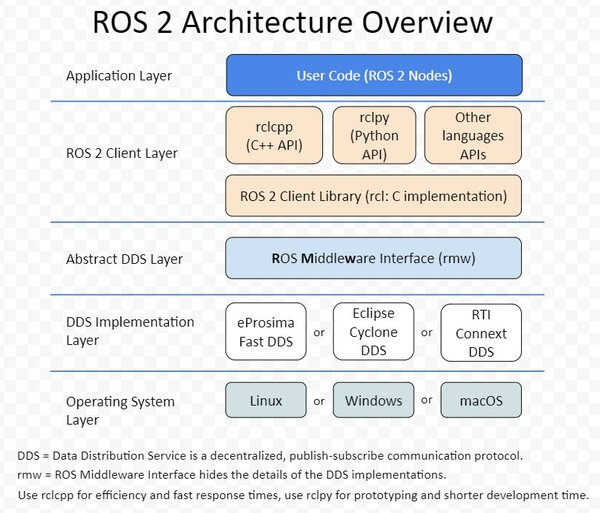
\includegraphics[width=0.8\textwidth]{"Bilder/ros-architecture.jpg"}
		\caption{ROS2 Architecture \cite{ros-2-architecture}}
		\label{fig:Background:Containers:Ros2_Architecture}					
	\end{figure}
	
	\subsection{ROS2 Nodes (Application layer)}
	\label{Grundlagen:ROS2:ROS2Nodes}

	In ROS distributed applications are typically designed as entities referred to as nodes. Each Node in ROS is supposed to be responsible for a single, modular function. In a Robotic Control System, sensors (lidar, camera), motion controllers (motors for movement), and algorithm components (route planners) can each be nodes.  A node can send and receive data to and from other nodes via topics, services, actions, or parameters.
	ROS 2 separates the node concept from the process structure at the operating system level. Multiple nodes can be created within a process as desired, and these nodes can independently interact with other nodes. All nodes in the system can run on a single computer or they can be distributed and run on multiple computers.


	\paragraph[ROS2]{ROS2 Communication Patterns}
	\label{Grundlagen:ROS2:CommunicationPatterns}

	The nodes communicate with each other via topics, service calls, and actions. Topic-based Communication is based on a publish-subscribe architecture, where the data generated and published by a node can be subscribed to by more than one node, and likewise, a Topic can produce data for more than one node. 
	The distributed architecture of the topic topology offers improvements in terms of performance and fault tolerance. Additionally, the extensive quality of service(QoS) features in the DDS middleware layer make ROS-2 architecture more robust and enable developers to use it in an industrial- /real-life application.

	A comprehensive robotic system has several nodes working together in harmony. In ROS 2 a single executable (C++ program, Python program, etc.) can hold one or more nodes in them. This network of ROS 2 elements running simultaneously and processing data is referred to as a ROS graph. It includes all executables and the connections between them.



	\begin{figure}[H]
		\centering
		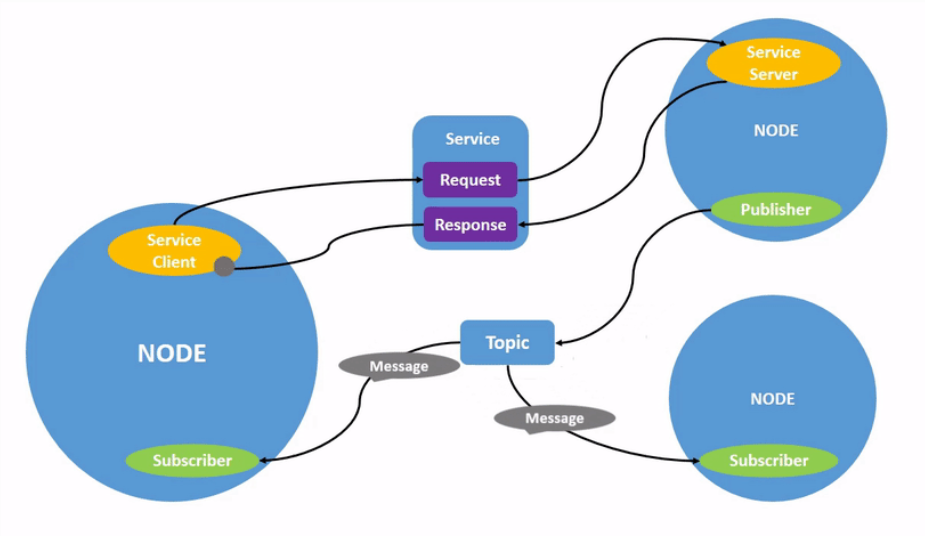
\includegraphics[width=0.8\textwidth]{"Bilder/ros-nodes.png"}
		\caption{ROS2 Communication Pattern \cite{ros2Basic}}
		\label{fig:Background:Ros2Nodes}					
	\end{figure}

	\begin{labeling}{Messages:}
		\item [Messages:] 
		A message is a data file that is sent via a communication channel called. Messages in ROS 2 are of great importance for interoperability. A publisher sends its message to a specific topic. This topic can be subscribed to by one or more subscribers. Several publishers can send messages to a topic and several subscribers can receive them. The communication in messages is unidirectional. A topic must use a message type that is known to all participants. There are predefined standard message types that are supplied with the ROS2 installation. Custom message types can be defined in a .msg- file. A message can contain other message definitions and can be extended using this pattern.\cite*{ros2Tutorials}
		
		\item [Topics:] 
		Topics act as virtual communication channels (bus) through which data is moved between nodes and consequently between various components of the system. Topics aren't just one-to-one connections moreover, they can be many-to-one, one-to-many, and many-to-many connections. Topics are a key element in realizing Publish-Subscribe architecture.
		Topics define the name and data structure used. Each topic in ROS2 is also an instance that can store historical message data in that topic.

		\item [Service:] 
		Two-way communication in ROS2 is made possible with services. A request is sent to a service server, which then responds to the request sent by the service client. A single service communication channel can contain several service clients but only one service server. The service server and service client must be both able to recognize the message type used. Custom service message types can be defined with a .srv file. This file defines the request and the response of service communication. A service can contain other service message definitions.
		\begin{figure}[H]
			\centering
			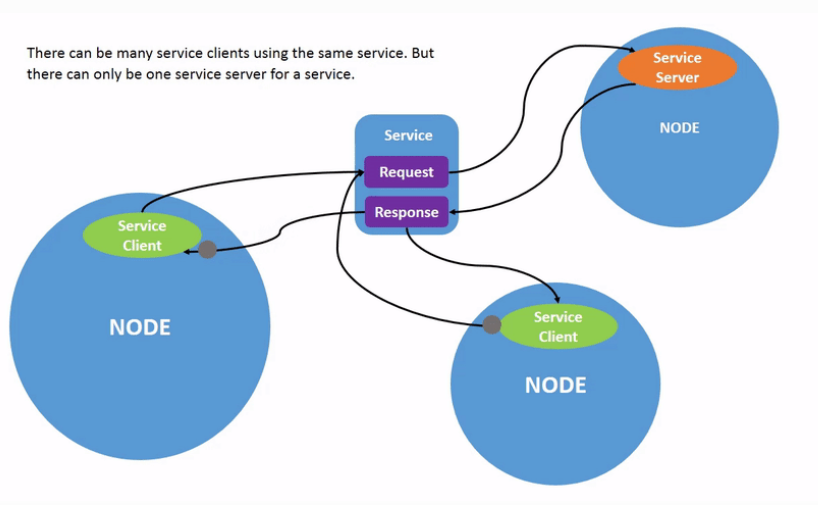
\includegraphics[width=0.8\textwidth]{"Bilder/ros-services.png"}
			\caption{ROS2 Services \cite{ros2Tutorials}}
			\label{fig:Background:Ros2Services}					
		\end{figure}
		
		\item [Action:]
		Actions are an advanced communication pattern in ROS2 that's designed for long-running tasks. They are made up of three parts: a goal, feedback, and result.
		Topics and services are the building blocks of Actions. Their functionality is similar to that of services, with the difference that actions are interruptible (they can be individually ended during execution). Unlike services, which only return a single response, they provide constant feedback.
		
		Actions use a client-server model, similar to the publisher-subscriber model. An "action client" node sends a goal to an "action server" node, which acknowledges the goal and returns a stream of feedback and a result. 

		\begin{figure}[H]
			\centering
			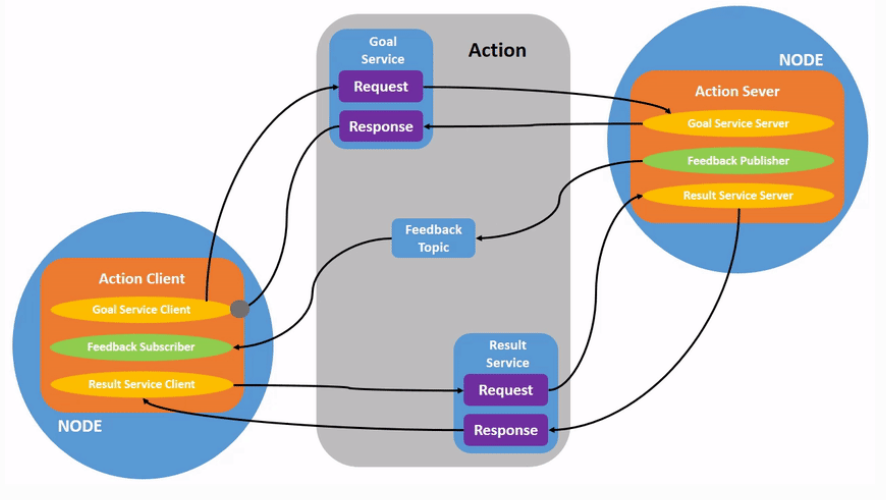
\includegraphics[width=0.8\textwidth]{"Bilder/ros-actions.png"}
			\caption{ROS2 Actions \cite{ros2Tutorials}}
			\label{fig:Background:Ros2Actions}					
		\end{figure}

		Figure \ref{fig:Background:Ros2Actions} gives an overview of the inner workings of an Action. The action client makes a Goal Request, which after processing can either be accepted or rejected by the action server. In case, the Goal Request is accepted it is forwarded to the action client. Then a user-defined function is called that executes the desired task of the action server. This Function continuously sends its current status or other custom information as feedback to the action client. Upon completion of the task and achievement of the defined goal, the action server sends the corresponding result response. Within an action communication channel, there can be several action clients, but only one action server. The action message type used must be recognized by all the participants in advance. Own action message types can be defined with a .action file. This contains the definition of Goal, Request, and Feedback. Other message definitions can be used from an existing action definition.		
		
	\end{labeling}

	\subsection{ROS2 Client Library}
	\label{Grundlagen:ROS2:ROS2ClientLibrary}
	Client libraries are the APIs that users can use to implement their ROS code. Client libraries give users access to ROS concepts such as nodes, themes, services, etc. Client libraries come in a variety of programming languages, so users can write ROS code in the language that best suits their application.

	Nodes written with different client libraries can exchange messages with each other because all client libraries implement code generators that allow users to interact with ROS interface files in the respective language.

	\subsection{ROS Middleware Interface}
	\label{Grundlagen:ROS2:ROSMiddlewareInterface}

	
	\subsection{Important ROS2 Concepts}
	\label{Grundlagen:ROS2:Concepts}

		
		The \text{ROS DOMAIN ID}\\
		About different ROS 2 DDS/RTPS vendors\\	
		About logging and logger configuration\\
		About ROS 2 client libraries\\
		About ROS 2 interfaces\\
		About parameters in ROS 2\\
		About topic statistics\\
		Introspection with command line tools\\
		About Composition\\
		On the mixing of ament and catkin (catment)\\

	\subsection{ROS2 Web Bridge}
	\label{Grundlagen:ROS2:2WebBridge}
		
	\subsection{roslibjs}
	\label{Grundlagen:ROS2:RosLibJS}
	
	

	\subsection{DDS}
	\label{Grundlagen:DDS}
		- Grundlage für Kommunikation von ROS2\\
		- Realisiert die eigentliche Kommunikation\\
		- Wenn das hier geht, geht auch ROS2!
		- Verschiedene Systemanbieter, näher wird RTI und Fastrtps untersucht: https://ros.org/reps/rep-2000.html  (Beide TIER 1)
		
	
	\section{Ros Lifecycle nodes}
	\label{Grundlagen:ROS2:Lifecycle}
	Having a managed lifecycle for nodes allows for better control over the state of the ROS system. This ensures that in a ROS2 Robotics System all components have been correctly instantiated before allowing a component to perform its behavior. It also allows nodes to be restarted or replaced online.

	A managed node has a known interface, executes according to a known lifecycle state machine. This allows the application (node) developer to decide how to implement various managed lifecycle functions while securing compatibility with other lifecycle nodes.\\
	
	The base functionality of a managed lifecycle node is described using a state machine illustrated in figure \ref*{fig:Background:Ros2LifecycleStateMachine}.\\

	\textit{"A state machine is a mathematical abstraction used to design algorithms. A state machine reads a set of inputs and changes to a different state based on those inputs. A state is a description of the status of a system waiting to execute a transition. A transition is a set of actions to execute when a condition is fulfilled or an event received."} \cite*{statemachineDef}\\

	There are 4 primary states (colored blue in figure \ref*{fig:Background:Ros2LifecycleStateMachine}):
	\begin{itemize}
		\item Unconfigured
		\item Inactive
		\item Active
		\item Finalized
	\end{itemize}
	In addition, there are 6 transition states, which are intermediate states during a requested transition(colored in yellow in figure \ref*{fig:Background:Ros2LifecycleStateMachine} ):
	\begin{itemize}
		\item Configuring
		\item CleaningUp
		\item Activating
		\item Deactivating
		\item ShuttingDown
		\item ErrorProcessing
	\end{itemize}
	There are 7 transitions exposed to the lifecycle management interface, which can be invoked only when the necessary conditions are met. These conditions are described in detail in the next section. The table below lists these transitions with the corresponding behavior invoked during their execution.
	\begin{table}[H]
		\centering
		\rowcolors{1}{}{gray!25}
		\caption{Availabe Transitions}
		\label{tab:Valid transitions}
		\begin{tabular}{|p{2cm}|p{9cm}|}
			\toprule
			Transition & Description\\
			\midrule
			create & with this transition the node is instantiated, but will not run any code beyond the constructor. On successful execution of the constructor the node is in Unconfigured state. \\
			configure & \textit{onConfigure()} callback is called\\
			cleanup & \textit{onCleanup()} callback is called\\
			activate & \textit{onActivate()} callback is called\\
			deactivate & \textit{onDeactivate()} callback is called\\
			shutdown & \textit{onShutdown()} callback is called\\
			destroy & with this transition the node is destroyed (deallocated). The node is completely removed from the system. \\
			\bottomrule
		\end{tabular}
	\end{table}

	\begin{figure}[H]
		\centering
		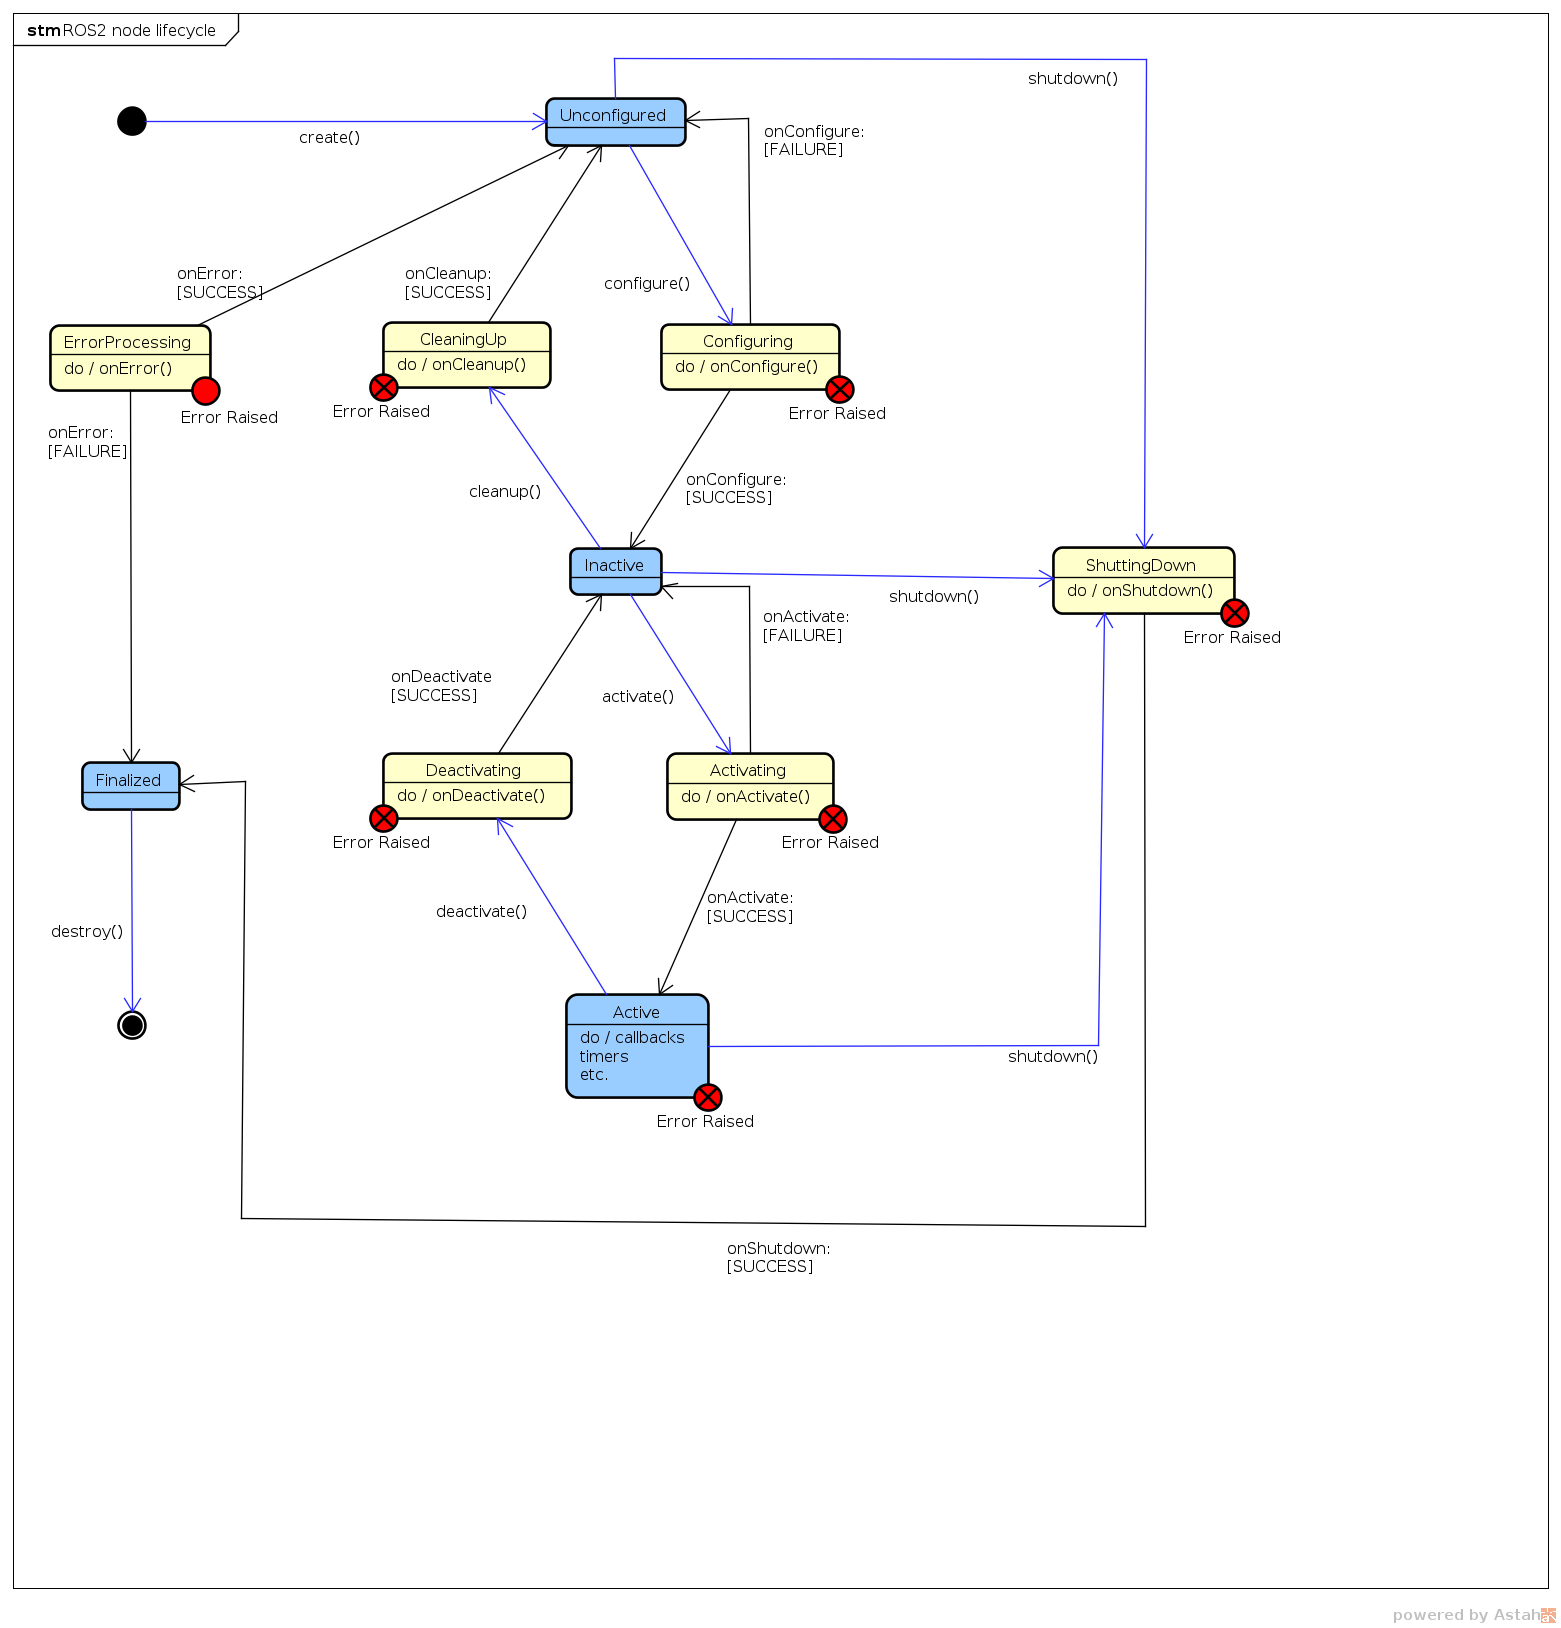
\includegraphics[width=0.95\textwidth]{"Bilder/ros_lifecycle.png"}
		\caption{ROS2 Lifecycle Statemachine \cite{ros-2-lifecycle}}
		\label{fig:Background:Ros2LifecycleStateMachine}					
	\end{figure}

	\subsection{Primary States}	
	The transition from a primary state requires an action of an external monitoring process, except in the case of an error triggered in the 3rd primary ("active") state.
	\begin{labeling}{Unconfigured:::::}
		\item[\textbf{Unconfigured}] This is the starting state of the state machine. When a node is instantiated, it finds itself in this lifecycle state. In case of any unexpected error, a node can be returned to this state. In this state, it is expected that there is no saved state. From this state the following transitions via corresponding transition states are availabe:
		\begin{table}[H]
			\centering
			% \rowcolors{1}{}{gray!25}
			\label{tab:Valid transitions}
			\begin{tabular}{|p{3cm}|p{3cm}|}
				\toprule
				Transition via & Final state\\
				\midrule
				configure & Inactive  \\
				shutdown & Finalized \\
				\bottomrule
			\end{tabular}
		\end{table}

		\item[\textbf{Inactive}] This state represents a node that is not currently operating. The main purpose of this state is to allow reconfiguration of a node (modifying configuration parameters, adding and removing topic publications/subscriptions, etc.) without changing its behavior during operation. In this state, the node does not read topics, process data, respond to functional service requests, etc. In the inactive state, all data arriving in managed topics is not read or processed. 
		
		Data storage is subject to the configured QoS policy for the topic. Any managed service requests to a node that is in the inactive state will not be answered (they will fail immediately for the caller). From this state the following transitions via corresponding transition states are availabe:
		\begin{table}[H]
			\centering
			% \rowcolors{1}{}{gray!25}
			\label{tab:Valid transitions}
			\begin{tabular}{|p{3cm}|p{3cm}|}
				\toprule
				Transition via & Final state\\
				\midrule
				shutdown & Finalized  \\
				cleanup & Unconfigured \\
				activate & Active \\
				\bottomrule
			\end{tabular}
		\end{table}

		\item[\textbf{Active}] It is the central state of the node's lifecycle. In this state, the node performs all processing, responds to service requests, reads and processes data, generates output, etc. All the important user functionality should be implemented in this state.  

		When an error occurs in this state that cannot be handled by the node/system, the node enters the ErrorProcessing state. From this state the following transitions via corresponding transition states are availabe:
		\begin{table}[H]
			\centering
			% \rowcolors{1}{}{gray!25}
			\label{tab:Valid transitions}
			\begin{tabular}{|p{3cm}|p{3cm}|}
				\toprule
				Transition via & Final state\\
				\midrule
				 deactivate & Inactive  \\
				 shutdown & Finalized \\
				\bottomrule
			\end{tabular}
		\end{table}

		\item[\textbf{Finalized}] In this state, the node ends its execution immediately before its deallocation. This state is always final, the only transition from here for a node is to be destroyed and completely removed from the system.

		The main purpose of this state is to support debugging and introspection. A failed node remains visible for introspection in the system and can potentially be examined by debugging tools before being destroyed. If a node is started in a respawn loop or there are known reasons for the cycling into this state, the supervising monitoring process can automatically destroy and recreate the node based on a predefined policy. From this state the following transitions via corresponding transition states are availabe:
		\begin{table}[H]
			\centering
			% \rowcolors{1}{}{gray!25}
			\label{tab:Valid transitions}
			\begin{tabular}{|p{3cm}|p{3cm}|}
				\toprule
				Transition via & Final state\\
				\midrule
				 destroy & Deallocated  \\
				\bottomrule
			\end{tabular}
		\end{table}

	\end{labeling}

	\subsection{Transition States} 
	Application-specific logic is executed in the transition states to determine if the requested transition was successful. The lifecycle management software is notified of success or failure via the lifecycle management interface before transitioning to another state.
	\begin{labeling}{ErrorProcessing:::::}
		\item[\textbf{Configuring}] In this transition state, the node's \textit{onConfigure()} callback is invoked to allow the node to load its configuration and make any necessary changes to its settings. Configuring a node typically involves tasks that need to be done once during the node's lifetime, such as allocating permanent memory buffers and setting up topic publications/subscriptions that do not change. The node uses this to set up all the resources it needs to keep throughout its lifetime (whether it is active or inactive). 
		From this state the following transitions are availabe:
		\begin{table}[H]
			\flushright
			% \rowcolors{1}{}{gray!25}
			\label{tab:Valid transitions}
			\begin{tabular}{|p{8.5cm}|p{3cm}|}
				\toprule
				Transition condition & Final state\\
				\midrule
				onConfigure callback succeeds & Inactive  \\
				onConfigure callback fails with an error code that can be handled by the node/system & Unconfigured \\
				onConfigure callback fails with an error that cannot be handled by the node/system  & ErrorProcessing \\
				\bottomrule
			\end{tabular}
		\end{table}

		\item[\textbf{CleaningUp}] In this transition state, the node's \textit{onCleanup()} callback is invoked, which is expected to clear all states and return the node to a functionally equivalent state as when it was first created. If the clean-up cannot be performed successfully, the method moves on to ErrorProcessing.
		From this state the following transitions are availabe:
		\begin{table}[H]
			\flushright
			% \rowcolors{1}{}{gray!25}
			\label{tab:Valid transitions}
			\begin{tabular}{|p{8.5cm}|p{3cm}|}
				\toprule
				Transition condition & Final state\\
				\midrule
				onCleanup callback succeeds & Unconfigured \\
				onCleanup callback fails with an error that cannot be handled by the node/system  & ErrorProcessing \\
				\bottomrule
			\end{tabular}
		\end{table}

		\item[\textbf{Activating}] In this transition state, the node's \textit{onActivate()} callback is invoked to allow the node to make the final preparations before starting execution. This may include obtaining resources necessary when the node is active(e.g. accessing the hardware). Ideally, no time-consuming operations should be made in this callback (e.g. a lengthy hardware initialization).
		From this state the following transitions are availabe:
		\begin{table}[H]
			\flushright
			% \rowcolors{1}{}{gray!25}
			\label{tab:Valid transitions}
			\begin{tabular}{|p{8.5cm}|p{3cm}|}
				\toprule
				Transition condition & Final state\\
				\midrule
				onActivate  callback succeeds & Active \\
				onActivate callback fails with an error that cannot be handled by the node/system  & ErrorProcessing \\
				\bottomrule
			\end{tabular}
		\end{table}

		\item[\textbf{Deactivating}] In this transition state, the node's \textit{onDeactivate()} callback is invoked, which is expected to do any cleanup necessary to start execution, and is supposed to reverse the changes made by \textit{onActivate()} callback .
		From this state the following transitions are availabe:
		\begin{table}[H]
			\flushright
			% \rowcolors{1}{}{gray!25}
			\label{tab:Valid transitions}
			\begin{tabular}{|p{8.5cm}|p{3cm}|}
				\toprule
				Transition condition & Final state\\
				\midrule
				onDeactivate callback succeeds & Inactive \\
				onDeactivate callback fails with an error that cannot be handled by the node/system  & ErrorProcessing \\
				\bottomrule
			\end{tabular}
		\end{table}

		\item[\textbf{ShuttingDown}] In this transition state, the node's \textit{onShutdown()} callback is invoked, which is expected to do any cleanup necessary before destruction of the node. It can be transitioned into from any Primary State except Finalized. The originating state is passed to this state as a parameter .
		From this state the following transitions are availabe:
		\begin{table}[H]
			\flushright
			% \rowcolors{1}{}{gray!25}
			\label{tab:Valid transitions}
			\begin{tabular}{|p{8.5cm}|p{3cm}|}
				\toprule
				Transition condition & Final state\\
				\midrule
				onShutdown callback succeeds & Finalized \\
				onShutdown callback fails with an error that cannot be handled by the node/system  & ErrorProcessing \\
				\bottomrule
			\end{tabular}
		\end{table}

		\item[\textbf{ErrorProcessing}] This state exists in order to be able to clear any unhandled errors.  All error processing functionality should be implemented in this state. This state can be transitioned into from any state where user code is executed. In case of successful error handling, the node can return to the Unconfigured state. If complete clean-up is not possible, the node must fail, and transition to the Finalised state. Transitions to ErrorProcessing can be triggered by errors in callbacks as well as by other methods within a callback or an uncaught exception.
		From this state the following transitions are availabe:
		\begin{table}[H]
			\flushright
			% \rowcolors{1}{}{gray!25}
			\label{tab:Valid transitions}
			\begin{tabular}{|p{8.5cm}|p{3cm}|}
				\toprule
				Transition condition & Final state\\
				\midrule
				onError callback succeeds & Unconfigured \\
				onError callback fails & Finalized \\
				\bottomrule
			\end{tabular}
		\end{table}

	\end{labeling}

	\subsection{Management Interface}
	A managed node is exposed to the ROS ecosystem through the following interface. This interface can be used by applications that perform the actual management. This interface is independent of the lifecycle status of individual nodes and is thus not be subject to any communication restrictions.

	A managed node or lifecycle node has a common pattern which it inherits from a container class that loads a managed node implementation from a library and, through a plug-in architecture, automatically exposes the required management interface by implementing callback methods. 

	A lifecycle node does not inherit from the regular \lstinline{rclcpp::node::Node} but from\\  \lstinline{rclcpp_lifecycle::LifecycleNode}. Every child of LifecycleNodes has a set of callbacks provided. These callbacks go along with the applied state machine attached to them. These callbacks are:

\begin{lstlisting}[language=cpp,
	caption={Transition Callbacks}, 
	label={code:TransitionCallbacks}]
	rclcpp_lifecycle::node_interfaces::
	LifecycleNodeInterface::CallbackReturn
	on_configure(const rclcpp_lifecycle::State & previous_state)

	rclcpp_lifecycle::node_interfaces::
	LifecycleNodeInterface::CallbackReturn
	on_activate(const rclcpp_lifecycle::State & previous_state)

	rclcpp_lifecycle::node_interfaces::
	LifecycleNodeInterface::CallbackReturn
	on_deactivate(const rclcpp_lifecycle::State & previous_state)

	rclcpp_lifecycle::node_interfaces::
	LifecycleNodeInterface::CallbackReturn
	on_cleanup(const rclcpp_lifecycle::State & previous_state)

	rclcpp_lifecycle::node_interfaces::
	LifecycleNodeInterface::CallbackReturn
	on_shutdown(const rclcpp_lifecycle::State & previous_state)

\end{lstlisting}

These management services can be implemented via attributes and method calls (for local management) and via ROS messages and topics/services (for remote management). In the case of providing a ROS middleware interface, specific topics placed in a suitable namespace are used. Each possible management transition is provided as a ROS service which can be called directly with the ros2 command-line interface. The service reports whether the transition was completed successfully. Following is a list of available services which maybe called from ros CLI or RosLibJS (ROS2 JavaScript API). 

\begin{lstlisting}[language=JavaScript]
	// Available Services :
	// /lifecycle_joytovel/change_state
	// /lifecycle_joytovel/describe_parameters
	// /lifecycle_joytovel/get_available_states
	// /lifecycle_joytovel/get_available_transitions
	// /lifecycle_joytovel/get_parameter_types
	// /lifecycle_joytovel/get_parameters
	// /lifecycle_joytovel/get_state
	// /lifecycle_joytovel/get_transition_graph
	// /lifecycle_joytovel/list_parameters
	// /lifecycle_joytovel/set_parameters
	// /lifecycle_joytovel/set_parameters_atomically
\end{lstlisting}

\subsection{Lifecycle management CLI} ROS2 developers have developed a basic CLI to interact with the lifecycle nodes and control their specific behaviours. 
It offers following functionalities and can be used as described below.
\begin{lstlisting}[language=bash,
	% caption={dockerfile_startup}, 
	label={code:DockerTestumgebung}]
	
	usage: ros2 lifecycle <command> <options>

	Various lifecycle related sub-commands
	Commands:
		get    Get lifecycle state for one or more nodes
		list   Output a list of available transitions
		nodes  Output a list of nodes with lifecycle
		set    Trigger lifecycle state transition
\end{lstlisting}

Get current lifecycle state
\begin{lstlisting}[language=bash,
	% caption={dockerfile_startup}, 
	label={code:DockerTestumgebung}]
	
	usage: ros2 lifecycle get [-h] [--spin-time SPIN_TIME] [--no-daemon][--include-hidden-nodes]                 [node_name]

	Get current lifecycle state
	
	positional arguments:
	node_name             Name of the ROS node
\end{lstlisting}

Trigger lifecycle state transition
\begin{lstlisting}[language=bash,
	% caption={dockerfile_startup}, 
	label={code:DockerTestumgebung}]
	
	usage: ros2 lifecycle set [-h] [--spin-time SPIN_TIME] [--no-daemon][--include-hidden-nodes] node_name transition

	Trigger lifecycle state transition

	positional arguments:
	node_name             Name of the ROS node
	transition            The lifecycle transition
\end{lstlisting}

Output a list of available transitions
\begin{lstlisting}[language=bash,
	% caption={dockerfile_startup}, 
	label={code:DockerTestumgebung}]
	
	usage: ros2 lifecycle list [-h] [--spin-time SPIN_TIME] [--no-daemon][--include-hidden-nodes] [-a] node_name

	Output a list of available transitions

	positional arguments:
	node_name             Name of the ROS node
	
\end{lstlisting}

Default values for transitions:
\begin{lstlisting}[language=bash,
	% caption={dockerfile_startup}, 
	label={code:DockerTestumgebung}]
	# Reserved [0-9], publicly available transitions.
	# When a node is in one of these primary states, these transitions can be
	# invoked.

	# This transition will instantiate the node, but will not run any code beyond
	# the constructor.
	uint8 TRANSITION_CREATE = 0


	# configuration and conduct any required setup.
	uint8 TRANSITION_CONFIGURE = 1

	# node to load its configuration and conduct any required setup.
	uint8 TRANSITION_CLEANUP = 2

	# The node's callback onActivate will be executed to do any final preparations
	# to start executing.
	uint8 TRANSITION_ACTIVATE = 3

	# The node's callback onDeactivate will be executed to do any cleanup to start
	# executing, and reverse the onActivate changes.
	uint8 TRANSITION_DEACTIVATE = 4

	# This signals shutdown during an unconfigured state, the node's callback
	# onShutdown will be executed to do any cleanup necessary before destruction.
	uint8 TRANSITION_UNCONFIGURED_SHUTDOWN  = 5

	# This signals shutdown during an inactive state, the node's callback onShutdown
	# will be executed to do any cleanup necessary before destruction.
	uint8 TRANSITION_INACTIVE_SHUTDOWN = 6

	# This signals shutdown during an active state, the node's callback onShutdown
	# will be executed to do any cleanup necessary before destruction.
	uint8 TRANSITION_ACTIVE_SHUTDOWN = 7

	# This transition will simply cause the deallocation of the node.
	uint8 TRANSITION_DESTROY = 8

	# Reserved [10-69], private transitions
	# These transitions are not publicly available and cannot be invoked by a user.
	
	# Reserved [90-99]. Transition callback success values.
	# These return values ought to be set as a return value for each callback.
	# Depending on which return value, the transition will be executed correctly or
	# fallback/error callbacks will be triggered.

	# The transition callback successfully performed its required functionality.
	uint8 TRANSITION_CALLBACK_SUCCESS = 97

	# The transition callback failed to perform its required functionality.
	uint8 TRANSITION_CALLBACK_FAILURE = 98

	# The transition callback encountered an error that requires special cleanup, if
	# possible.
	uint8 TRANSITION_CALLBACK_ERROR = 99

	##
	## Fields
	##

	# The transition id from above definitions.
	uint8 id

	# A text label of the transition.
	string label
			
\end{lstlisting}


	\section{Vue JS}
	\label{Grundlagen:Vue}
	Vue is described as a progressive web framework. This means that it adapts to the needs of the developer. While other frameworks require a complete adoption of a technology by a developer or team and often require an existing application to be rewritten because of certain framework-specific conventions. Vue can be introduced to an application with a simple script tag and can grow with requirements, from a small web component to managing the entire view layer. Vue is a scalable JavaScript framework for building user interfaces. Unlike other frameworks, Vue is designed from the ground up to be incrementally customizable. The core library is view-only and easily integrates with other libraries or existing projects. In combination with modern tools and additional libraries, Vue is capable of running sophisticated single-page applications \cite{Vue019:Intro:Online}.
	It is not necessary to have prior knowledge of Webpack, Babel, npm or the like to get started with Vue. HTML, CSS, and the basics of JavaScript are enough to get started with Vue.

	The leap from a pure HTML and CSS-based website to a sophisticated web application is very simple and can be learned during the development process. This is a strong selling point, especially in the current ecosystem of JavaScript front-end frameworks and libraries, which makes newcomers and even experienced developers feel lost in the ocean of possibilities and choices. The goal of Vue is to be able to create reasonable web applications with minimal prior knowledge.
	
	\subsection{Main Features of Vue}
	\label{Grundlagen:VueFeatures}
	Together with React and Angular, Vue is one of the most popular frameworks in the web development landscape. The following features characterize the Vue framework:


	
	\paragraph*{Components:} Vue components extend basic \gls{HTML} elements to encapsulate reusable code. The Vue component system is an abstraction that enables the creation of large applications from small, self-contained, and often reusable components.
	\paragraph*{Templates:} Vue.js uses an HTML/\gls{CSS}-based template syntax. Vue compiles the templates into Virtual DOM render functions. In combination with the reactivity system, Vue can intelligently determine the minimum number of components that need to be updated. This minimizes the number of DOM manipulations when the application changes state.
	\paragraph*{Reactivity:} Vue has a reactivity system that uses pure JavaScript objects and optimizes rendering. Each component keeps track of its reactive dependencies during rendering. This allows the system to intelligently and optimally re-render the components.
	\paragraph*{Integration:} It is very easy to integrate Vue into existing projects or to add third-party libraries to Vue. All JavaScript libraries that use ES6+ can be used within Vue. For example, Bootstrap, Material Design, ThreeJS, Web Sensors API, etc.  Vue also offers the possibility to use TypeScript instead of JavaScript.
	\cite{VueGuide:Online}


	\subsection{Vue in comparision to Angular und React}
	\label{sec:VueAngularReact}
	Vue borrowed some of the Angular templating syntaxes but removed the complex stack that Angular required. This made it very powerful. Vue took many good ideas from React, especially the virtual DOM.  But Vue implements it with a kind of automatic dependency management that tracks which components are affected by a change in the state so that only those components are re-rendered when the state property changes. In React, on the other hand, if any part of the state that affects a component changes, that component is re-rendered, and thus any associated child components are also re-rendered. This is an advantage for Vue in terms of usability and performance enhancement \cite{VueComparision:Online}.

\begin{table}[H]
	\centering
	\caption{Vue vs React vs Angular \cite{ComparisonVue:Online}}
	% \rowcolors{2}{}{gray!25}
	\label{tab:table_VueJS}
	\begin{tabular}{{p{3cm}|p{3cm}|p{3cm}|p{3cm}}}
    \toprule
    Criterion & 
\includegraphics[width=0.05\textwidth]{Bilder/img/vue.png} & 
\includegraphics[width=0.05\textwidth]{Bilder/img/react.png} & 
\includegraphics[width=0.05\textwidth]{Bilder/img/angular.png}\\
     & Vue & React & Angular\\
    \midrule
    Focus & Usability & Flexibility & TypeScript \\
    Complexity & Low & Medium & High\\
    Size & 80 KB & 100 KB & 500+ KB\\
    Release & 2014 & 2013 & 2010 \\
    Developed by & Evan You & Facebook & Google \\
    Language & JavaScript & JavaScript & TypeScript\\
    Model & virtual DOM & virtual DOM & \gls{MVC}\\
    Supported by & Open Source & Facebook & Google \\
    Latest version & 2.6.11 & 16.13.1 & 9.1.11\\
		\bottomrule
	\end{tabular}
\end{table}


\subsection{Structure of a Vue.js project}
\label{sec:StructureofVue.jsProject}
Vue has a very intuitive project structure. In addition to the core framework, it includes a lot of utilities that make front-end development with Vue very enjoyable.
Like most JavaScript projects, NodeJS is used for Vue development. Vue provides the core library and the add-on utilities via \texttt{\textbf{\gls{npm}}}.

\paragraph{NodeJS} is a JavaScript runtime environment based on Chrome's V8 JavaScript engine. It allows JavaScript code to be executed outside of a web browser. NodeJS allows developers to use JavaScript to write command-line tools and execute scripts server-side to generate dynamic web page content before the page is sent to the user's web browser. NodeJS supports unifying web application development around a single programming language, rather than using different languages for server-side and client-side scripting \cite{NodeJS:Online}.

\paragraph{npm (node package manager)} is the largest software registry in the world. Open-source developers from every continent use npm to share and access packages, and many organizations also use npm to manage private development \cite{NPM:Online}.

\paragraph*{Vue-CLI:} Vue provides an official CLI(Command Line Interface) for quickly setting up modern single-page applications. It provides a comprehensive build setup for a modern front-end workflow. It takes just minutes to get up and running with hot-reload, lint-on-save, and production build.

\paragraph{Installation}
The installation of the required packages is done with NodeJS and npm. The following commands must be executed to create a basic Vue application:
\begin{itemize}
	\item Install the Vue CLI globally:
	\begin{lstlisting}[language=bash]
		npm install -g @vue/cli
	\end{lstlisting}
	\item The Vue-\gls{CLI} is used to create a new Vue project.
	\begin{lstlisting}[language=bash]
		vue create example_vue_app
	\end{lstlisting}
	This opens a CLI where the desired configuration for a Vue project can be set.
	\item To start the development server, the following command is executed:
	\begin{lstlisting}[language=bash]
		npm run serve
	\end{lstlisting}
	\item To create a production build for the app, the following command is executed:
	\begin{lstlisting}[language=bash]
		npm run build
	\end{lstlisting} 
\end{itemize} 


A typical Vue project with Vue-Router and Vuex has the following structure:

\begin{table}[H]
	\centering
	\caption{Structure of the project folder}
	\rowcolors{1}{}{gray!25}
	\label{tab:table_VueJS}
	\begin{tabular}{{p{4cm}p{9cm}}}
		\toprule
		Files/Folders & Description\\
		\midrule
    	public/index.html & This is the main app file loaded by the browser. The file contains only a simple HTML tag in the body: \texttt{ \textcolor{red}{<div id=app> </div>}}. 
		This is the element that attaches the Vue application to the DOM. \\
		\hline
		src/main.js & This is the JavaScript file responsible for configuring the Vue.js application. It is also used to register all third-party packages. \\
		\hline
		src/App.vue & This is the root component that contains the HTML content that is displayed to the user. \\
		\hline
		/package.json & In this file npm stores the names and versions of the package it installed. \\
		\hline
		src/components/ & This folder contains the additional components. \\
		\hline
			src/assets/ & This folder is used to store static content, such as images. \\
		\hline
			src/router/ & This folder contains the implementation of Vue-Router. \\
			\hline
			src/store/ & The folder contains the implementation of Vuex-Store. \\
		\bottomrule
	\end{tabular}
\end{table}

\subsection{Vue Instance} Every Vue application begins by creating a new Vue instance (root instance) with the Vue function. When a Vue instance is created, it adds to Vue's reactivity system all the properties found in its data object(described in table \ref{tab:table_data}).  All \texttt{Vue.js} internal modules and external plugins to be used are imported in the \texttt{(main.js)} file with ES6(ECMAScript 2015) import syntax ('import'). The dependencies are defined as global parameters and are accessible by all components.  
% A typical VueJS project has a structure as shown in \ref{fig:vue_project_structure}. 
In the main.js file, the main Vue component (\texttt{App.vue}) is registered. 

\begin{lstlisting}[language=JavaScript, caption=main.js]
    import Vue from 'vue'
    import App from './App'
    import router from './router'

    // Root Instance
    new Vue({
        el: '#app',
        router,
        template: '<App/>',
        components: { App }
    })

\end{lstlisting}

\subsection{Vue Component}The most important criterion for choosing this framework \texttt{(Vue.js)} is the modularity of the individual components. The components are one of the strongest features of \texttt{Vue.js}. They allow basic HTML elements to be extended to encapsulate reusable code. At a high level, components are custom elements to which the \texttt{Vue.js} compiler attaches a specific behavior \cite{Vue019:Intro:Online}. Each component is defined in a file with \texttt{.vue} extension. The definition contains an HTML-based template that specifies the design of the component and the JavaScript code that specifies all other functionality or behavior of the component. Each component is also a Vue instance.

Typically, a Vue.js app is organized in a tree of nested components. For example, it consists of components for a header, sidebar, and content area, each containing other components for navigation links, blog posts, etc. The component architecture simplifies such nesting.

\begin{figure}[H]
  \centering
  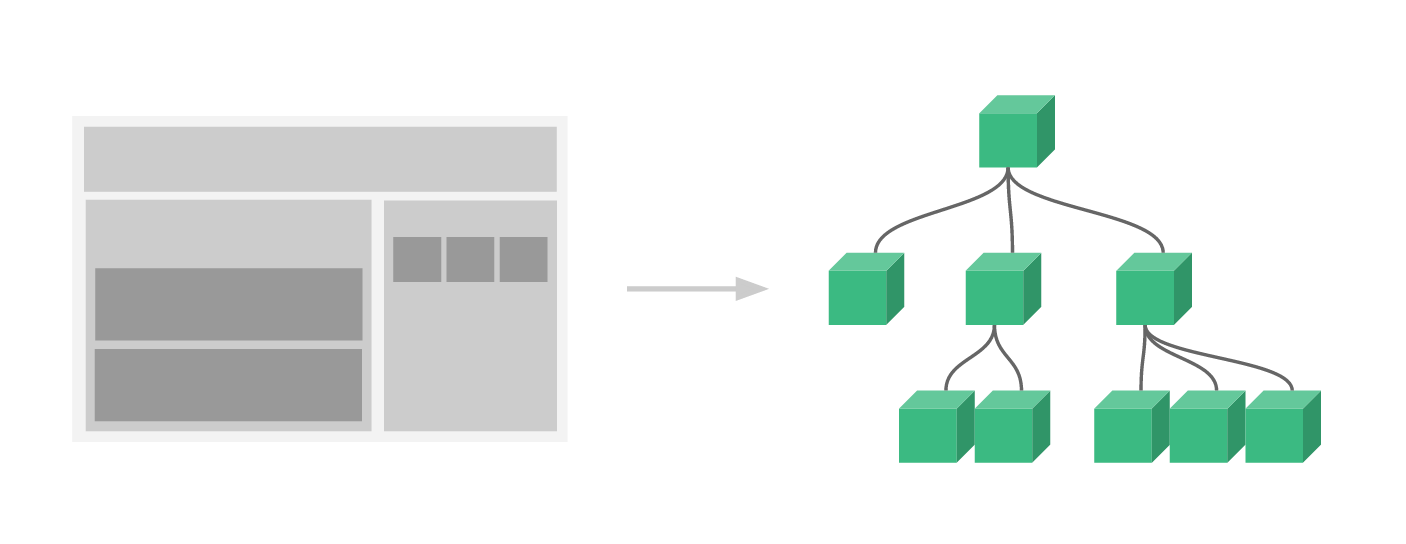
\includegraphics[width=0.9\textwidth]{Bilder/img/components.png}  
  \caption{ \textit{Organization of Componenten} \cite{VueComponents:Online}}%
\label{fig:OrganisationvonKomponenten}
\end{figure}

% Die grundlegende Struktur einer \texttt{Vue.js} Komponente ist im Listing \ref{lst:label} dargestellt. 

The template element contains the HTML template and the script element contains the JavaScript part of the component.
\begin{labeling}{Template element::}
	\item [Template element:] The design of the user interface is implemented in this element. Standard HTML and CSS technology are used for this. User-defined HTML elements, as well as HTML elements from external plug-ins, can be integrated very easily. The HTML-based template syntax of Vue.js allows binding the rendered DOM declaratively to the data of the underlying Vue instance. All Vue. js templates are valid HTML.
	
	The simplest form of data binding is text interpolation using the \textit{mustache} syntax (double curly braces):
	\begin{lstlisting}[language=html,label={lst:label}, caption=Templateelement]
        <template>
            <div>
                <h1>Data: {{ beispielData }}</h1>
                <BeispielComponent/>
            </div>
        </template>    
        \end{lstlisting}
		\item [Script element:] This element contains the implementation of the desired functionalities of the component with \texttt{VueJS} specific construct. Further components can be imported and registered here. These are then available in the template element, which allows the nesting of components to be realized.
	\begin{lstlisting}[language=JavaScript,label={lst:label}, caption=Skriptelement]
        
        <script>
          import BeispielComponent from 'components/BeispielComponent'
          export default {
            components: {
              BeispielComponent
            },
            props : [],
            data () {
              return {
                beispielData: 'Beispiel String'
              }
            },
            methods: {
                beispielFunction: function () { }
            },
            computed: {
            }
          }
        </script>
        
        \end{lstlisting}
\end{labeling}


The most important parts of a component are described in the table \ref{tab:table_data}.
\begin{table}[H]
	\centering
	\caption{Parameters responsible for data manipulation}
	\rowcolors{1}{}{gray!25}
	\label{tab:table_data}
	\begin{tabular}{{p{1.7cm}p{4cm}p{8cm}}}
		\toprule
		Parameters & Type & Description\\
        \midrule
        components & [key: string]: Object &This is a list of custom components to be used. The custom or external components are imported with \texttt{\textcolor{purple}{import}} command to import them from the ES6 specification.\\
		data & Object or Function & This is a JavaScript object or function that allows the storage of the necessary attributes for the component. Within the component, the original data object can be accessed with \texttt{\textcolor{purple}{this.data}} directive can be accessed.\\
		props & Array\(<string>\) or Object & This is a list/hash of attributes intended to hold data from the parent component. It has a simple array-based syntax and an alternative object-based syntax that allows advanced configurations such as type checking, custom validation and default values. \\
        methods & [key: string]: Function & This is a list of methods that allow the realisation of different functionalities of the component.  All methods can be called within the component as a standard JavaScript method.\\
        computed & [key: string]: Function & This is a list of methods that will be called automatically when the reactive dependencies change. The attributes within these parameters are cached and only recomputed on reactive dependency changes. \\
		\bottomrule
	\end{tabular}
\end{table}


\subsection{instance lifecycle hooks} When created, each Vue instance goes through a series of initialization steps, e.g. it needs to set up data observation, compile the template, including the instance in the DOM and update the DOM when the data changes. In parallel, it also runs functions called lifecycle hooks that allow users to add their functions at certain stages of the instance lifecycle. This allows very precise control of the behavior of individual components.

For example, the \textit{created} hook can be used to execute code after an instance has been created. Other hooks are called at different stages of the instance lifecycle, such as. \textit{mounted}, \textit{updated} and \textit{destroyed}. The figure \ref{fig:OrganisationOfComponents} illustrates the details of the complete lifecycle hook.

\begin{figure}[H]
  \centering
  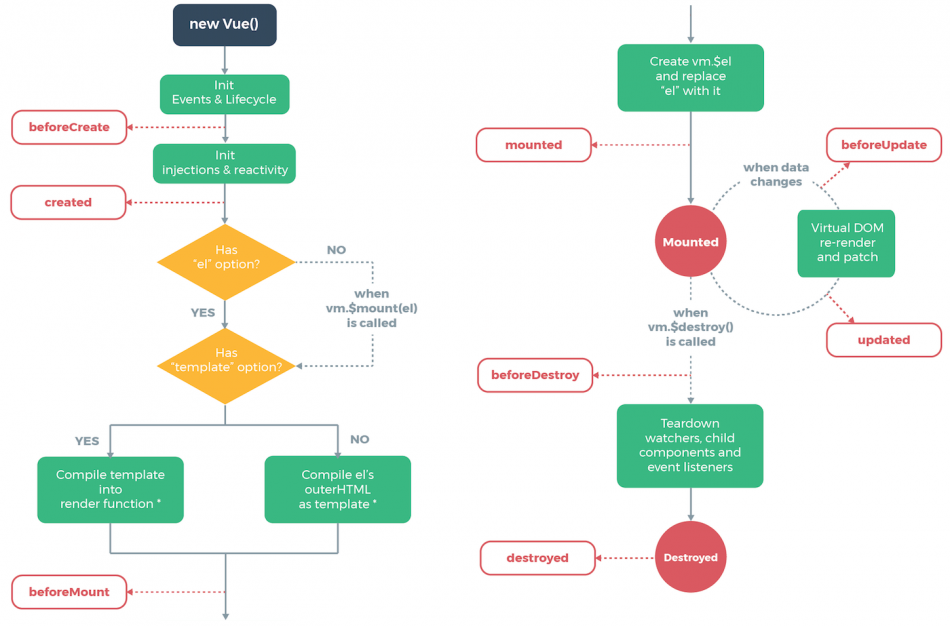
\includegraphics[width=1\textwidth]{Bilder/img/lifecycle_.png}  
  \caption{ \textit{Vue Instance-Lifecycle Hooks} \cite{InstancVue:Online}}%
\label{fig:OrganisationOfComponents}
\end{figure}



\subsection{Vuex }
\label{sec:Vuex}
Vuex is the official state management library for Vue. Its job is to exchange data between components in a Vue application.

Components in a Vue application can have their state. For example, an input field stores the data entered in it locally. Components can be input fields or a whole page. It becomes very costly to exchange state data between nested components.

Vuex provides central storage(Vuex store) for the state, and the state can be changed by calling functions defined in the Vuex store.
Each component that depends on a particular piece of state accesses it via a getter function on the Vuex store, ensuring synchronization of data. Vuex-Store is a kind of temporary database for a particular application session \cite{VueGuide:Online}.


\subsection{Vue Router }
\label{sec:Vue Router}

In a web application, a router is a part that synchronizes the currently displayed view with the contents of the browser address bar.

A router is needed when \gls{URL}s need to be synchronized with the views in an application. This is a very common need, and all major modern frameworks now allow routing to be managed.   Vue Router is part of the Vue core library and handles route management in a Vue application \cite{VueGuide:Online}.


\section{Nginx}
\label{Grundlagen:Nginx}
Nginx, pronounced like "engine-ex", is an open-source web server that is now also used as a reverse proxy, HTTP cache, and load balancer. It is one of the most used web servers along with the Apache HTTP server.\cite{nginxIntro}

This section describes the basics of NGINX (start, stop reload configuration), the structure of the configuration file and describes the process of setting up NGINX to serve out static content.

\subsection{Starting, Stopping, and Reloading Configuration}
Nginx has a single master process and several worker processes. The master process reads and evaluates the configuration and manages the worker processes. The worker processes operate the real processing of HTTP requests. Nginx uses an event-based model and operating system-dependent means to efficiently allocate requests among the worker processes. The number of worker processes is set in the configuration file.\cite{nginxIntro}


\subsection{Structure of Configuration File }
The configuration file is named by default nginx.conf and placed in the directory \textit{"/usr/local/nginx/conf", "/etc/nginx", or "/usr/local/etc/nginx"}. Nginx consists of modules that are controlled by directives defined in the configuration file. Directives are split into simple directives and block directives. A simple directive is made up of the name and parameters separated by spaces and ends with a semicolon (;). A block directive ends with a sequence of additional arguments surrounded by curly braces. A block directive that contains other directives inside curly braces, is called a context (examples: events, http, server, and location). Directives that are outside contexts in the configuration file are in the main context. The directives events and http are in the main context. The server directive is inside the http directive and location inside the server. For comments, a hashtag \lstinline{(#)} sign is used.\cite*{nginxIntro}

\subsection{Serving Static Content}

		
\chapter{Previous Work}

Masterarbeit von Christoph (Für DDS und Routing service)